
\newcommand{\Cyclus}{\textsc{Cyclus}\xspace}%
\subsection{Predicting the Past: Spent Fuel Mass Validation}
\begin{frame}
  \frametitle{Predicting the Past: Spent Fuel Mass Validation}

\begin{block}{What is Predicting the Past? }
Use published data regarding 112 commercial nuclear reactors in the U.S. to create a \Cyclus simulation of the U.S. nuclear fuel cycle.
\end{block}


\begin{block}{Who}
Gwendolyn Chee, UIUC Graduate Student Researcher
\end{block}

\begin{block}{Where}
        \url{https://github.com/arfc/transition-scenarios} 
\end{block}
\end{frame}

\begin{frame}
\begin{block}{Current Work}
A comparison of spent fuel mass and isotopic compositions from the Predicting 
the Past \Cyclus output and spent nuclear fuel inventory from the U.S 
Department of Energy sponsored Unified Database\cite{peterson_unf-st&dards_2017} was conducted. This work has been submitted to ANS Winter 2018.
\end{block}

\begin{figure}[htbp!]
                \begin{center}
                        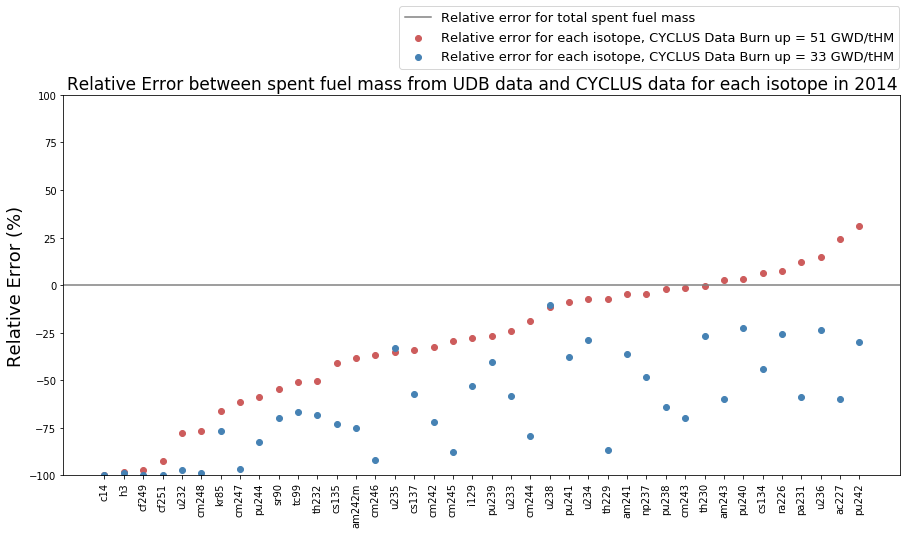
\includegraphics[height=0.7\textheight]{./images/relative_error_2014.png}
                        \caption{Relative error between cyclus prediction and 
                                CURIE data}
                \end{center}
        \end{figure}

\end{frame}


\subsection{Transition Benchmark}
\begin{frame}
\begin{block}{What is the Transition Benchmark}
        Publish Cyclus contirbution to the ``Standardized Verification of Fuel 
        Cycle Modeling'' paper (Feng et al.)
\end{block}

\begin{block}{Who}
Jin Whan Bae, UIUC Graduate Student Researcher
\end{block}

\begin{block}{Where}
        \url{https://github.com/arfc/transition-scenarios} 

\end{block}

\end{frame}

\begin{frame}

\begin{figure}[htbp!]
    \begin{center}
        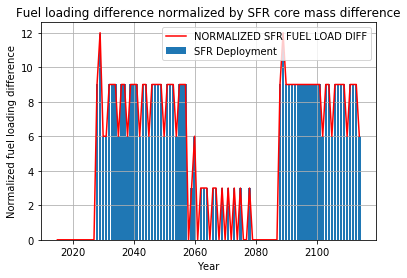
\includegraphics[scale=0.5]{./images/fuel_load_diff_norm.png}
    \end{center}
        \caption{Difference of annual fresh \gls{SFR} fuel loading rates (Cyclus - Benchmark) normalized by the core mass difference of an \gls{SFR} due to fractional batch size.}
    \label{fig:fuel_load_diff_norm}
\end{figure}

\end{frame}
\begin{frame}
\begin{figure}[htbp!]
    \begin{center}
        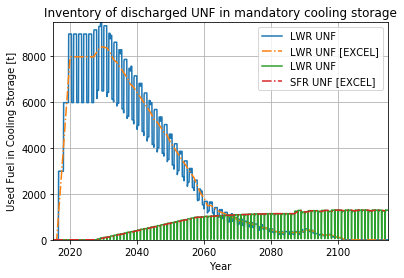
\includegraphics[scale=0.5]{./images/fuel_discharge_monthly.png}
    \end{center}
        \caption{Inventory of discharged UNF in mandatory cooling storage.}
    \label{fig:fuel_discharge_monthly}
\end{figure}

\end{frame}
